% !Mode::"TeX:UTF-8"
\documentclass[a4paper, 10pt]{article}
\usepackage{amssymb}
\usepackage{geometry}
\usepackage{graphicx}
\usepackage{fancyhdr}
\usepackage{setspace}
\usepackage{pdfpages}
\usepackage{listings}
\usepackage{amsthm}
\usepackage{authblk}
\usepackage{amsmath}
\usepackage{url}
\usepackage{hyperref}

\graphicspath{{./figure/}}

\geometry{left=2.5cm,right=2.5cm,top=2.5cm,bottom=2.5cm}

%\author{Chi Zhang\\\\Department of Computer Science\\\\University of Southern California}
\title{\textbf{Deep Reinforcement Learning for Portfolio Management}\thanks{Instructor: Joseph J. Lim}}
\author[]{Chi Zhang}
\author[]{Limian Zhang}
\author[]{Corey Chen}
\affil[]{Department of Computer Science}


\begin{document}

  \maketitle                     %generate the title
  \begin{spacing}{1.2}
    \section{Problem Definition}
    \subsection{Notations}
    In this project, we would like to manage portfolio by distributing our investment into a number of stocks based on the market. We define our environment similar to this paper \cite{DBLP:journals/corr/JiangXL17}.
    Concretely, we define $N$ to be the number of stocks we would like to invest.
    Without losing generality, at initial timestamp, we assume our total investment volume is 1 dollar. We define \emph{close/open relative price vector} as:
    \begin{equation}
    y_t=[1, \frac{v_{1,t, close}}{v_{1,t, open}}, \frac{v_{2,t, close}}{v_{2,t, open}},\cdots,\frac{v_{N,t,close}}{v_{N,t, open}}]
    \end{equation}
    where $\frac{v_{i, t, close}}{v_{i, t, open}}$ is the \emph{relative price} of stock $i$ at timestamp $t$. 
    Note $y[0]$ represents the relative price of cash, which is always 1. We define \emph{portfolio weight vector} as:
    \begin{equation}
    w_t=[w_{0,t}, w_{1, t}, \cdots, w_{N, t}]
    \end{equation}
    where $w_{i,t}$ represents the fraction of investment on stock $i$ at timestamp $t$. Note that $w_{0,t}$ represents the fraction of cash that we maintain. Then the profit after timestamp $T$ is:
    \begin{equation}
    \label{profit}
    p_T=\prod_{t=1}^{T}y_t\cdot w_{t-1}
    \end{equation}
    where $w_0=[1, 0, \cdots, 0]$. If we consider a trading cost factor $\mu$, then the trading cost of each timestamp is:
    \begin{equation}
    {\mu}_t=\mu\sum{|\frac{y_t \odot w_{t-1}}{y_t \cdot w_{t-1}} - w_{t}|}
    \end{equation}
    where $\odot$ is element-wise product. Then equation~\ref{profit} becomes:
    \begin{equation}
    \label{profit_mu}
    p_T=\prod_{t=1}^{T}(1-\mu_t) y_t\cdot w_{t-1}
    \end{equation}
    
    \subsection{Key Assumptions and Goal}
    To model real world market trades, we make several assumptions to simplify the problems:
    \begin{itemize}
      \item We can get any information about the stocks before timestamp $t$ for stock $i$. e.g. The previous stock price, the news and tweets online.
      \item Our investment will not change how the market behaves.
      \item The way we calculate profit in equation~\ref{profit} can be interpreted as: At timestamp $t$, we buy stocks according to the \emph{portfolio weight vector} $w_{t-1}$ computed by history data at \textbf{open} price and sell all the stocks at \textbf{close} price. This may not be true in practice because you will not always be able to \textbf{buy/sell} the stock at \textbf{open/close} price.
    \end{itemize}
    The \textbf{goal} of portfolio management is to maximum $p_T$ by choosing portfolio weight vector $w$ at each timestamp $t$ based on history stock information.
    
    \subsection{MDP formulation}
    \subsubsection{State and Action}
    We define state $s_t$ as $o_t$, where $o_t$ is the obseration of timestamp $t$. As the time goes by, the impact of history data decreases. Thus, we only consider the history price and news in a fixed window length $W$. Hence,
    \begin{equation}
    o_t=[\vec{v_{1,t}},\vec{v_{2,t}},\cdots,\vec{v_{N,t}}]
    \end{equation}
    where
    \begin{align}
    v_{i,t} &=\begin{bmatrix}
    v_{i,t-W} \\
    v_{i,t-W+1} \\
    \vdots \\
    v_{i,t-1}
    \end{bmatrix}
    \end{align}
    and $N$ is the number of stocks. The action $a_{t}$ is just \emph{portfolio weight vector} $w_{t}$. Note that this is a continuous state and action space problem. We try to directly solve it in continuous space instead of using discretization in previous work \cite{cs229_stanford_portfolio, cs229_stanford_trading}. Essentially, we want to train a policy network $\pi_\theta(a_t|o_t)$.
    \subsubsection{State Transition}
    The underlining state evolution is determined by the market, which we don't have any control. What we can get is the observation state, which is the price. Since we will collect history price of various stocks, $o_t$ is given by the dataset instead of $o_{t-1}$.\\
    \subsubsection{Reward}
    Instead of having reward 0 at each timestamp and $p_T$ at the end, we take logarithm of equation~\ref{profit_mu}:
    \begin{equation}
    \log{p_T}=\log{\prod_{t=1}^{T}\mu_t y_t\cdot w_{t-1}}=\sum_{t=1}^{T}\log(\mu_t y_t\cdot w_{t-1})
    \end{equation}
    Thus, we have $\log(\mu_t y_t\cdot w_{t-1})$ reward each timestamp, which avoids the sparsity of reward problem.\\
    
    \subsection{Datasets}
    \textbf{Stocks used:}
    We use 16 target stocks from NASDAQ100 that we feel are representative of different sectors in the index fund. They include "AAPL", "ATVI", "CMCSA", "COST", "CSX", "DISH", "EA", "EBAY", "FB", "GOOGL", "HAS", "ILMN", "INTC", "MAR", "REGN" and "SBUX".\\
    \textbf{Price Data:}
    We collected history price of the stocks from 2012-08-13 to 2017-08-11. The price on each day contains open, high, low and close. We use 2012-08-13 to 2015-08-12 as training data and 2015-08-13 to 2017-08-11 as testing data.\\
    \textbf{News Data:}
    We gather all tweets referencing the stocks from 2016-03-28 to 2016-06-15.\\
    \textbf{Additional Testing Data:}
    As another form of backtesting, we randomly select 16 stocks from NASDAQ100 the network has never seen and test whether the network generalizes.
    
    \section{Methods}
    We mainly consider model-free approach in our project. First, we train a predictor given a fixed history window length $W$ of price and news. With the predicted price, we can train a policy network $\pi_{\theta}(a_t|s_t)$ to maximize our portofolio value at the end of the trading period. Note that in practice, they are trained end-to-end instead of separately.
    
    \subsection{Data Preprocessing}
    Instead of using the raw price data, we normalize the history price as $(\frac{close}{open} - 1)\times scale$. There are two main advantages:
    \begin{enumerate}
      \item The history price are all in the same scale regardless of their actual price.
      \item Since the final portfolio is determined by the close/open ratio of each timestamp, it serves as a better feature compared with raw price.
    \end{enumerate}
    The \emph{scale} factor is heuristically set to 100 in our experiments.
    
    \subsection{Predictor Network}
    
    
    
    \subsection{Optimal Action and Imitation Learning}
    If we have a perfect predictor, then we can ignore risk and just pick the best stock for each day. We greedily choose the stock with the highest close/open ratio (taking into account trading cost of changing stocks), buying as much as possible on the open and selling all at the close. Here is one such possible monotonically increasing output: 
    
    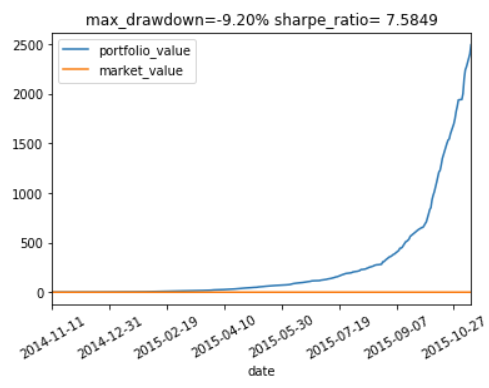
\includegraphics[scale=0.5]{Optimal_with_trading_cost.png}
    
    Then, we can train a model by imitating optimal action: we have as input the previous state $(o_t, a_{t-1})$, and as output label we compute to our next day's action. We will be using a CNN and LSTM to do this and compare the results. I believe this approach will yield good outcomes if the model can generalize to unseen data.
    
    \subsection{Deep Deterministic Policy Gradient (DDPG)}
    We applied similar reinforcement learning algorithm for continuous action space in this paper~\cite{DBLP:journals/corr/LillicrapHPHETS15}. However, we don't have any promising results yet. The main issue is that the model doesn't seem to be training because the action the actor network produces are all equally distributed weights. e.g. $[0.25, 0.25, 0.25, 0.25]$ if we have 3 stocks plus cash. I want to take some time to debug the network by seeing how the network is updated by the gradient at each step. Also, a key part is the exploration noise we added when sample actions. Currently, I just use uncorrelated Gaussian noise and the result is very bad. I would like to try parameter noise mentioned here \cite{DBLP:journals/corr/PlappertHDSCCAA17}. 
    
    
    \subsubsection{Critic Network Topology}
   
    
    
    \section{Results and Discussions}
    
    \section{Contribution}
    \textbf{Chi Zhang:} 
    \begin{itemize}
      \item Collect and preprocess stock price.
      \item Set up environment (OpenAI gym).
      \item Train DDPG model. (Doesn't work very well now, need to dig more)
    \end{itemize}
    \textbf{Corey Chen:}
    \begin{itemize}
      \item Compute optimal action
      \item Train CNN and LSTM policy network using imitation learning. (TODO)
    \end{itemize}
    \textbf{Limian Zhang:}
    \begin{itemize}
      \item Collect and preprocess tweets datasets.
      \item Predict future stock price based on history price and tweets data (TODO)
    \end{itemize}
    
    
%    
%    \begin{figure}
%      \centering
%      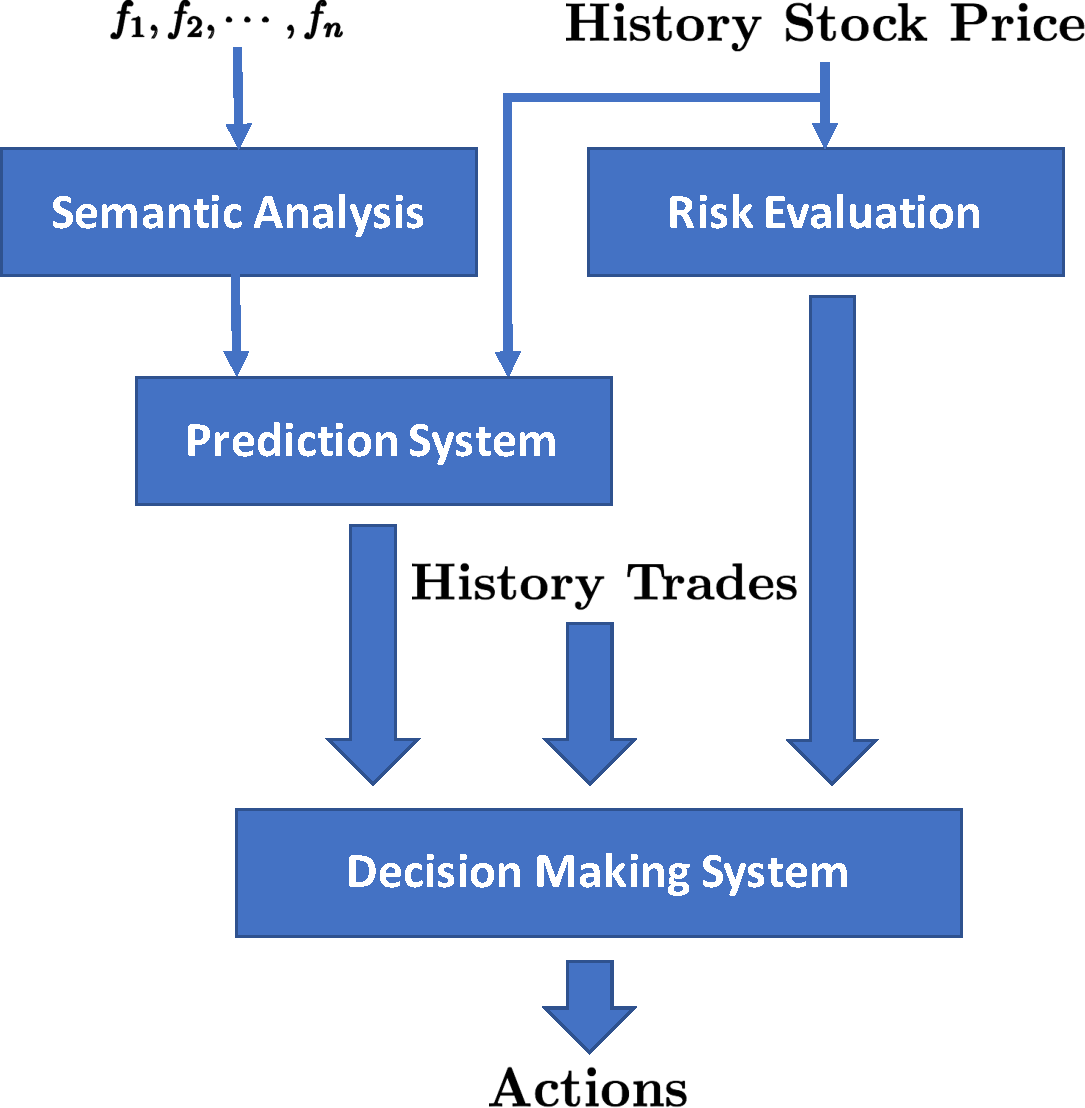
\includegraphics[width=0.4\textwidth]{diagram}
%      \caption{Digram of proposed approach}
%      \label{diagram_approach}
%    \end{figure}
    
    
  
  \end{spacing}  

  \bibliographystyle{IEEEtran}
  \bibliography{./bib/stock_prediction.bib}

\end{document}
